\documentclass[article]{jss}
\usepackage{rotating}
\usepackage{pdfpages}
\usepackage{booktabs}
\usepackage{setspace}

\author{Garrett Grolemund\\Rice University \And 
        Hadley Wickham\\Rice University}
\title{Dates and Times Made Easy with \pkg{lubridate}}

\Plainauthor{Garrett Grolemund, Hadley Wickham}
\Plaintitle{Dates and times made easy with lubridate}
\Keywords{dates, times, time zones, daylight savings time, \proglang{R}}
\Plainkeywords{dates, times, time zones, daylight savings time,  R}

%% publication information
%% \Volume{13}
%% \Issue{9}
%% \Month{September}
%% \Year{2004}
%% \Submitdate{2004-09-29}
%% \Acceptdate{2004-09-29}

\Address{
  Garrett Grolemund\\
  Rice University\\
  Houston, TX 77251-1892, United States of America\\
  E-mail: \email{grolemund@rice.edu}
}

\Abstract{
  This paper presents the lubridate package for \proglang{R}, which facilitates working with dates and times.  Date-times create various technical problems for the data analyst. The paper highlights these problems and offers practical advice on how to solve them using \pkg{lubridate}.  The paper also introduces a conceptual framework for doing math with date-times.
}

%\setstretch{2}
\begin{document}

\section{Introduction}

Date-time data can be frustrating to work with. It comes in many different formats, which makes recognizing and parsing it a challenge. Will our program handle the format that we have? If it does, we still face a slew of problems specific to date-times. How can we easily extract components of the date-times, such as years, months, or seconds? How can we effortlessly switch between time zones, or compare times from places that use daylight savings time (DST) with times from those that do not? Date-times create even more complications when we try to do math with them. Conventions such as leap years and DST make it unclear what we mean by ``one day from now" or ``exactly two years away."  Even leap seconds can disrupt a seemingly straight forward calculation.  This complexity affects other tasks too, such as constructing sensible tick marks for plotting date-time data.

While base \proglang{R} handles some of these problems, the syntax it uses is often confusing, uninviting, and difficult to remember. Moreover, the correct \proglang{R} code often changes depending on the class of date-time object being used. \pkg{lubridate} acknowledges these problems and makes it easier to work with date-time data in \proglang{R}. Specifically, \pkg{lubridate} helps users:

\begin{itemize}
   \item identify and parse date-time data, Section~\ref{sec:parsing} 
   
    \item extract and modify components of a date-time, such as years, months, days, hours, minutes, and seconds, Section~\ref{sec:accessors}
  
  \item perform accurate math on date-times, Section~\ref{sec:types}
    
  \item handle time zones and Daylight Savings Time, Sections~\ref{sec:tz}, and~\ref{sec:DST}, and
  
   \item construct pretty graphs with date-time data, Section~\ref{sec:pretty}, 
  
\end{itemize}

\pkg{lubridate} uses an intuitive user interface inspired by the date libraries of object oriented programming languages.  \pkg{lubridate} methods are compatible with a wide-range of common date-time objects. These include character strings, POSIXct, POSIXlt, Date, chron, fCalendar, zoo, xts, its, tis, timeSeries, fts, and tseries objects. Note that \pkg{lubridate} overrides the + and - methods for POSIXt, Date, and difftime objects in base \proglang{R}.\\

The time concepts introduced by \pkg{lubridate} are inspired by the \proglang{Java} based JODA time project, \url{http://joda-time.sourceforge.net/}. This paper demonstrates the convenient tools provided in the \pkg{lubridate} package and ends with a case study, which uses \pkg{lubridate} in a real life example.

\pkg{lubridate} can be downloaded at \url{http://cran.r-project.org/}. Its development site is \url{http://github.com/hadley/lubridate}.

\section{Motivation}

To see how \pkg{lubridate} simplifies things, consider a common scenario. We have a character string. We'd like to read it in as a date-time, extract the month, and change it to February (i.e. 2). On the left are the base \proglang{R} methods we'd use for these three tasks.  On the right are the \pkg{lubridate} methods.

\begin{center}
  \begin{tabular}{|p{7cm}|p{7cm}|}
    \hline
    \proglang{base R} & \pkg{lubridate}\\
    \hline
    \code{date <- as.POSIXct("01-01-2010", } & \code{date <- dmy("01-01-2010")}\\
    \indent \code{   format = "\%d-\%m-\%Y")} & \\
    & \\
    \code{as.numeric(format(date, "\%m"))} \# or  & \code{month(date)}\\
   \code{as.posixlt(date)$month + 1} &\\
    & \\
     \code{date <- as.POSIXct(format(date, } & \code{month(date) <- 2} \\
 \indent \code{   "\%Y-2-\%d"))} & \\
 \hline
\end{tabular}
\end{center}

Now we'll go a step further. We'll go back a day in time and display our new date in the Coordinated Universal time zone (UTC).

\begin{center}
  \begin{tabular}{|p{7cm}|p{7cm}|}
    \hline
     \proglang{base R} & \pkg{lubridate}\\
    \hline
    \code{seq(date, length = 2, by =}  & \code{date - days(1)} \\
    \indent \code{   "-1 day")[2]} & \\
   & \\
   \code{as.POSIXct(format(as.POSIXct(date),}  & \code{with_tz(date, "UTC")}\\
  \indent \code{    tz = "UTC"), tz = "UTC")} &\\
    \hline
\end{tabular}
\end{center}

\pkg{lubridate} makes basic date-time manipulations much more straight forward. Plus, the same \pkg{lubridate} methods work for all of the popular date-time object classes (\code{Date}, \code{POSIXt}, \code{chron} ... ).

Table 1 provides a more complete comparison between \pkg{lubridate} methods and base \proglang{R} methods. It shows how \pkg{lubridate} can simplify each of the common date time tasks presented in RNews Volume 4/1, June 2004. It also provides a useful summary of \pkg{lubridate} methods.
% Always a good idea to show some examples right off the bat.  This helps
% people understand why they should bother reading the paper

\includepdf[angle=90]{comparison-table}

\section{Parsing date-times}
\label{sec:parsing}

We can read dates into R using the \code{ymd()} series of functions provided by \pkg{lubridate}. The letters y, m, and d correspond to the year, month, and day elements of a date-time. To read in a date, choose the function name that matches the order of elements in your date-time object. For example,\\

\code{R> ydm("2010-31-12")}\\
\code{[1] "2010-12-31 CST"}\\

or

\code{R> ymd(c("2010.12.31", "2011.01.01"))}\\
\code{[1] "2010-12-31 CST"}\\


These functions create a POSIXct date-time object that matches the date described by the character string.  The functions automatically recognize the following separators: ``-", ``/", ``.", and ``" (i.e., no separators). When a \code{ymd()} function is applied to a vector of dates, \pkg{lubridate} will assume that all of the dates have the same order and the same separators. It will also print a message that tells the user which format was used to parse the dates. \code{ymd()} type functions also exist for times recorded with hours, minutes, and seconds. These functions make it simple to parse any date-time object that can be converted to a character string. See Table~\ref{tbl:parsers} for a complete list of \code{ymd()} type parsing functions. 

\begin{table}
  \begin{center}
  \begin{tabular}{ll}
  \toprule
  Order of elements in date-time & Parse function\\
  \midrule
  year, month, day & \code{ymd}\\
  year, day, month  & \code{ydm}\\
  month, day, year & \code{mdy}\\
  day, month, year & \code{dmy}\\
  hour, minute & \code{hm}\\
  hour, minute, second & \code{hms}\\
  year, month, day, hour, minute, second & \code{ymd.hms}\\
  \bottomrule
    
  \end{tabular}
  \end{center}
  \caption{Parse functions based on order of date-time elements.}
  \label{tbl:parsers}
\end{table}

\section{Manipulating date-times} 
\label{sec:accessors}

Every date-time is a combination of different elements, each with its own value. For example, most date-times include a year value, a month value, a day value, etc. Together, these elements specify the exact moment that the date-time refers to. We can easily extract each element of a date-time with the accessor function that has its name, as shown in Table~\ref{tbl:accessors}. For example,  if we save the current system time\\

\code{R> date <- now()}\\
\code{[1] "2010-02-25 09:51:48 CST"}\\

we can extract each of its elements.\\

\code{R> year(date)}\\
\code{[1] 2010}\\

\code{R> month(date)}\\
\code{[1] 2}\\

\code{R> minute(date)}\\
\code{[1]  51}\\


\begin{table}
  \begin{center}
  \begin{tabular}{ll}
  \toprule
  Date component & Accessor\\
  \midrule
  Year & \code{year()}\\
  Month & \code{month()} \\
  Week  &\code{week()} \\
  Day of year & \code{yday()} \\
  Day of month & \code{mday()}\\
  Day of week & \code{wday()}\\
  Hour & \code{hour()}\\
  Minute & \code{minute()}\\
  Second & \code{second()}\\
  Time Zone & \code{tz()}\\
  \bottomrule
    
  \end{tabular}
  \end{center}
  \caption{Date-time accessors used by lubridate.}
  \label{tbl:accessors}
\end{table}

We can also use any of the accessor functions to set the value of an element. This would also change the moment that the date-time refers to. For example,\\

\code{R> day(date) <- 5}\\
\code{[1] "2010-02-05 09:51:48 CST"}\\

changes our date to the fifth day of the month. We can also set the elements to more complicated values, e.g.\\

\code{R> minute(dates) <- mean(minute(dates))}\\

Note that if we set an element to a larger value than it supports, the difference will correctly roll over into the next higher element. For example,\\

\code{R> day(date) <- 30}\\
\code{[1] "2010-03-02 09:51:48 CST"}\\

We can use this to find the last day of a month:\\

\code{R> day(date) <- 1}\\
\code{R> month(date) <- month(date) + 1}\\
\code{R> day(date) <- day(date) - 1}\\
\code{[1] "2010-03-31 09:51:48 CDT"}\\


Lubridate also provides an update method for date-times.  This is useful if you want to change multiple attributes at once or would like to create a modified copy, instead of transforming in place.\\

\code{R> update(date, year = 2010, month = 1, day = 1)}\\
\code{[1] "2010-01-01 09:51:48 CST"}\\

Finally, we can also change dates by adding or subtracting units of time from them. For example, the methods below produce the same result.\\

\code{R> hour(date) <-  12 }\\
\code{[1] "2010-02-25 12:51:48 CST"}

\code{R> date + hours(3) }\\
\code{[1] "2010-02-25 12:51:48 CST"}\\

Notice that \code{hours()} (plural) is not the same function as \code{hour()} (singular). \code{hours()} creates a new object that allows us to do math with date-times. These objects are discussed in the next section. 

\section{Math with date-times}
\label{sec:types}
Doing math with date-times is more complicated than doing math with numbers, but it can be done accurately and easily with \pkg{lubridate}. What complicates math with date-times? Clock times are periodically re-calibrated to reflect astronomical conditions, such as the hour of daylight, or the Earth's tilt on its axis relative to the sun. We know these re-calibrations as daylight savings time, leap years, and leap seconds. Consider how one of these conventions might complicate a simple math operation. If today were January 1st, 2010 and we wished to know what day it would be one year from now, we could simply add 1 to the years element of our date.\\

January 1st, 2010 + 1 year = January 1st, 2011\\

Alternatively, we could add 365 to the days element of our date because a year is equivalent to 365 days. \\

January 1st, 2010 + 365 days = January 1st, 2011\\

Troubles arise if we try the same for January 1st, 2012. 2012 is a leap year, which means it has an extra day. Our two approaches above now give us different answers because the length of a year has changed.\\ 

January 1st, 2012 + 1 year = January 1st, 2013\\
January 1st, 2012 + 365 days = December 31st,  2012\\

At different moments in time, the lengths of months, weeks, days, hours, and even minutes will also vary. We can consider these to be \emph{relative} units of time; their length is relative to when they occur. In contrast, seconds always have a consistent length. Hence, seconds are \emph{exact} units of time.

Researchers may be interested in exact lengths, relative lengths, or both. For example, the speed of a physical object is most precisely measured in exact lengths. The opening bell of the stock market is more easily modeled with relative lengths.

\pkg{lubridate} allows math with both relative and exact units by introducing four new time related objects. These are \emph{instants}, \emph{intervals}, \emph{durations}, and \emph{periods}.  \pkg{lubridate} borrows instants, intervals, durations, and periods from the \proglang{JODA} time project. For more information about these concepts please visit the \proglang{JODA} time project at  \url{http://joda-time.sourceforge.net/}. 

\subsection{Instants}
\label{sec:instants}

An instants is a specific moments in time, such as January 1st, 2012. We create an instant, each time we parse a date into \proglang{R}. \\

\code{R> start_2012 <- ymd.hms("2012-01-01 12:00:00")}\\

\pkg{lubridate} does not create instant class objects. Instead, it recognizes any date-time object that refers to a moment of time as an instant. We can test if an object is an instant by using \code{is.instant()}. For example,\\

\code{R> is.instant(364)}\\
\code{[1] FALSE}\\

\code{R> is.instant(start_2012)}\\
\code{[1] TRUE}\\

We can easily round instants to the nearest minute, hour, month, etc. using \code{floor_date()}, \code{ceiling_date()}, and \code{round_date()}. For example,

\code{R> round_date(date, "day")}\\
\code{[1] "2012-01-02 00:00:00 CST"}\\

We can also capture the current time as an instant with the function \code{now()}, and the current day with the function \code{today()}.



\subsection{Intervals}
\label{sec:intervals}

Intervals, durations, and periods are all ways of recording time spans. Of these, intervals are the most simple. An interval is a period of time that occurs between two specific instants. The length of an interval is never ambiguous, because we know when it occurs. We can calculate the exact lengths of any unit of time that occurs during it. 

We can create interval objects by subtracting two instants or by using the command \code{new_interval()}.\\

\code{R> start_2011 <- ymd.hms("2011-01-01 12:00:00")}\\
\code{R> start_2010 <- ymd.hms("2010-01-01 12:00:00")}\\
\code{R> span <- start_2011 - start_2010}\\
\code{[1] 365 days beginning at 2010-01-01}\\

Unfortunately, since intervals are anchored to their start and end dates, they are not very useful for date-time math. It only makes sense to add an interval to its start date or to subtract it from its end date.\\

\code{R> start_2010 + span}\\
\code{[1] "2011-01-01 12:00 CST"}\\


\subsection{Durations}
\label{sec:durations}

If we remove the start and end dates from an interval, we will have a generic time span that we can add to any date. But how should we measure this length of time? If we record the time span in seconds, it will have an exact length since seconds always have the same length. We call such time spans \emph{durations}. Alternatively, we can record the time span in larger units, such as minutes or years. Since the length of these units varies over time, the exact length of the time span will depend on when it begins. These non-exact time spans are called \emph{periods} and will be discussed in the next section.

The length of a duration is invariant to leap years, leap seconds, and daylight savings time because durations are measured in seconds, which are also invariant to such phenomena. Hence, durations have consistent lengths and can be easily compared to other durations. Durations are the appropriate object to use when comparing time based attributes, such as speeds, rates, and lifetimes.

\pkg{lubridate} uses the \code{difftime} class from base \proglang{R} for durations. Additional \code{difftime} methods have been created to facilitate this. 

For large durations, it becomes inconvenient to describe the length in seconds. For example, not many people would recognize 31536000 seconds as the length of a standard year. For this reason, \pkg{lubridate} uses standard time units to display durations. However, these units are only estimates given for convenience. The underlying object is always recorded as a fixed number of seconds. Estimated units are created using the following relationships. A minute is 60 seconds, an hour 3600 seconds, a day 86400, a week 604800, and a year 31536000. Month units are not used because they are so variable.

Duration objects can be easily created with the helper functions 
\code{eyears()}, \code{eweeks()}, \code{edays()}, \code{eminutes()}, and  \code{eseconds()}. The e in the title stands for estimated. Each object creates a duration in seconds using the estimated relationships given above. The argument of each function is the number of estimated units we wish to include in the duration. For example,\\

\code{R> eminutes(1)}\\
\code{Duration of 1 mins}\\

\code{R> eseconds(60)}\\
\code{Duration of 1 mins \# 60 seconds = 1 estimated minute}\\

\code{R> eminutes(2)}\\
\code{Duration of 2 mins}\\

\code{R> c(1:3) * ehours(1) }\\
\code{Durations in hours}\\
\code{[1] 1 2 3}\\

Unlike intervals, durations can be added and subtracted to any instant object. For example,\\

\code{R> start_2011 + eyears(1)}\\
\code{[1] "2012-01-01 12:00:00 CST"}\\

\code{R> start_2012 + eyears(1)}\\
\code{[1] "2012-12-31 12:00:00 CST"}\\

Durations can also be added to or subtracted from intervals and other durations. For example,\\

\code{R> eweeks(1) + edays(6) + ehours(2) + eminutes(1.5) + eseconds(3)}\\
\code{Duration of 1.869201 weeks}\\

We can also create durations from intervals using \code{as.duration()}. 

\code{R> as.duration(span)}\\
\code{Duration of 1 year}\\


\subsection{Periods}
\label{sec:periods}

Unlike durations, periods have a relative length. Periods record a time span in units larger than seconds, such as years, months, weeks, days, hours, minutes, or a combination of these. For convenience, we can also create a period that only uses seconds, but such a period would have the same properties as a duration. We construct periods with the helper functions \code{years()}, \code{months()}, \code{weeks()}, \code{days()}, \code{minutes()}, and  \code{seconds()}.\\

\code{R> months(3)}\\
\code{[1] 3 months}\\

\code{R> months(3) + days(2)}\\
\code{[1] 3 months and 2 days}\\

These functions do not contain an e in their name, because they are no longer estimates. For example, \code{months(2)} always has the length of two months even though the length of two months will change depending on when the period begins. For this reason, we can not compute exactly how long a period will be in seconds until we know when it occurs. However, we can still do date-time math with periods. When we add or subtract a period to an instant, the period becomes anchored to the instant. The instant tells us when the period occurs, which allows us to calculate its exact length in seconds. 

In other words, we can use periods to accurately model clock times without knowing when events such as leap seconds, leap days, and DST changes occur.

\code{R> start_2011 + years(1)}\\
\code{[1] "2012-01-01 12:00:00 CST"}\\

\code{R> start_2012 + years(1)}\\
\code{[1] "2013-01-01 12:00:00 CST"}\\

We can also convert intervals to period objects with the function \code{as.period()}.\\

\code{R> as.period(span)}\\
\code{[1] 1 year}\\

Periods can be added to instants, intervals, and other periods, but not to durations.


In summary, math with date-times involves four types of objects: instants, intervals, durations, and periods. Table~\ref{tbl:date-math} describes which objects can be added to each other and what type of object will result.

\begin{table}
  \begin{center}
  \begin{tabular}{l|llll}
  & instant & interval & duration & period\\
  \hline
  instant & N/A & instant & instant & instant\\
  interval & instant & N/A & interval & interval\\
  duration & instant & interval & duration & N/A\\
  period & instant & interval & N/A & period\\
  \hline
    
  \end{tabular}
  \end{center}
  \caption{Object that results from adding two date-time objects}
  \label{tbl:date-math}
\end{table}

\section{Time zones}
\label{sec:tz}

Time zones are a way to give multiple names to the same instant. For example, ``2010-03-26 11:53:24 CDT" and ``2010-03-26 12:53:24 EDT" both describe the same instant. The first shows how the instant is labeled in the United States' central time zone (CDT). The second shows how the same instant is labelled in the United States' eastern time zone (EDT). Time zones complicate date-time data, but are useful for mapping clock time to local daylight conditions. When working with instants, it is standard to give the clock time as it appears in the Coordinated Universal time zone (UTC).  This saves calculations, but can be annoying if your computer insists on translating times to your current time zone.  It may also be inconvenient to discuss clock times that occur in a place unrelated to the data.

\pkg{lubridate} eases the frustration caused by time zones in two ways. We can change the the time zone in which an instant is displayed by using the function \code{with_tz()}. This changes how the clock time is displayed, but not the instant that is referred to. For example,\\

\code{R> date}\\
\code{[1] "2010-01-01 09:51:48 CST"}\\
\code{R> with_tz(date, "UTC")}\\
\code{[1] "2010-01-01 15:51:48 UTC"}\\

Occasionally, it is useful to keep the same clock time and change the time zone it is assigned to. This switch is accomplished with the \code{force_tz()} function. \code{force_tz()} does the opposite of \code{with_tz()}: it changes the instant that is displayed, but the clock time remains the same. For example, the code below moves us to a new instant that occurs 6 hours earlier.\\

\code{R> date}\\
\code{[1] "2010-01-01 09:51:48 CST"}\\
\code{R> force_tz(date, "UTC")}\\
\code{[1] "2010-01-01 09:51:48 UTC"}\\


\section{Daylight Savings Time}
\label{sec:DST}

In many parts of the world, the official clock time springs forward by one hour in the spring and falls back one hour in the fall. For example, in Houston, Texas a change in daylight savings time occurred at 2:00AM on March 14, 2010. The last instant before this change was 2010-03-14 01:59:59 CST.\\

\code{R> dst_time <- ymd.hms("2010-03-14  01:59:59")}\\
\code{[1] "2010-03-14 01:59:59 CST"}\\

One second later, Houston clock times read\\

\code{R> dst_time + eseconds(1)}\\
\code{[1] "2010-03-14 03:00:00 CDT"}\\

It seems that we gained an extra hour during that second, which is how daylight savings time works. We can completely avoid the changes in clock tim caused by daylight savings times by working with periods instead of durations. If we ever inadvertently try to create an instant that occurs in the one hour ``gap" between 2010-03-14 01:59:59 CST  and 2010-03-14 03:00:00 CDT, \pkg{lubridate} will return \code{NA} since such times are not available.

\section{Case Study 1}

The next two sections will work through some techniques using \pkg{lubridate}. First, we will use \pkg{lubridate} to calculate the dates of  holidays. Then we'll use \pkg{lubridate} to explore an example data set (\code{basketball}).

\subsection{Thanksgiving}
Some holidays, such as Thanksgiving (U.S.) and Memorial Day (U.S.) do not occur on fixed dates. Instead, they are celebrated according to a common rule. For example, Thanksgiving is celebrated on the fourth thursday of November. To calculate when Thanksgiving will be held in 2010, we can start with the first day of 2010.\\

\code{R> date <- ymd("2010-01-01")}\\
\code{[1] "2010-01-01 CST"}\\

We can then add months, until we get to November.\\

\code{R> date + months(10)}\\
\code{[1] "2010-11-01 CDT"}\\

Next, we add thursdays until we get to the fourth thursday in November.\\

\code{R> date + months(10) + thursdays(4)}\\
\code{[1] "2010-11-25 CST"}\\

If we wanted the dates of thanksgiving for the next four years, we could do that too.\\

\code{R> date + years(c(0:3)) + months(10) + thursdays(4)}\\
\code{[1] "2010-11-25 CST" "2011-11-24 CST" "2012-11-22 CST" "2013-11-28 CST"}\\

This would also work if we reversed the order of \code{years(c(0:3))} and \code{months(10)}, but we'd get a trivial result if we placed \code{months(10)} or \code{years(c(0:3))} after \code{thursdays(4)}, i.e.\\

\code{R> date + months(10) + thursdays(4) + years(c(0:3))}\\
\code{[1] "2010-11-25 CST" "2011-11-25 CST" "2012-11-25 CST" "2013-11-25 CST"}\\

Here we're asking \pkg{lubridate} to find one epoch and then calculate a sequence of years from that point. Before we constructed a sequence of years and then asked \pkg{lubridate} to find an epoch for each year.

\subsection{Memorial Day}
Memorial day also occurs according to a rule; it always occurs on the last monday of May. To calculate the date of Memorial day, we can again start with the first of the year.\\

\code{R> date <- ymd("2010-01-01")}\\
\code{[1] "2010-01-01 CST"}\\

Now, however, our holiday occurs in relation to the last day of the month instead of the first. So we add months until we get to June, and then subtract a day to get the last day of May.\\

\code{R> date + months(5) - days(1)}\\
\code{[1] "2010-05-31 CDT"}\\

To find the last monday of May, we subtract days until we get to the first monday, which happens to be May 31st.\\

\code{R> date + months(5) - days(1) - mondays(1)}\\
\code{[1] "2010-05-31 CDT"}\\


\section{Case Study 2}
Now let's explore the \code{basketball} data set. The \code{basketball} data set contains play by play statistics of every major league basketball game played in the 2008-2009 season. This data is from \url{http://www.basketballgeek.com/downloads/2009-2010/}. \\

\code{R> head(basketball)}\\

First we'll examine when during the year basketball games are held. We choose to use the \pkg{ggplot2} package to create our graphs. Please see \url{http://had.co.nz/ggplot2/} for more information about \pkg{ggplot2}.\\

\code{R> qplot(date, data = basketball, geom = "histogram", binwidth = 86400)}\\

\begin{figure}[htpb]
  \centering
  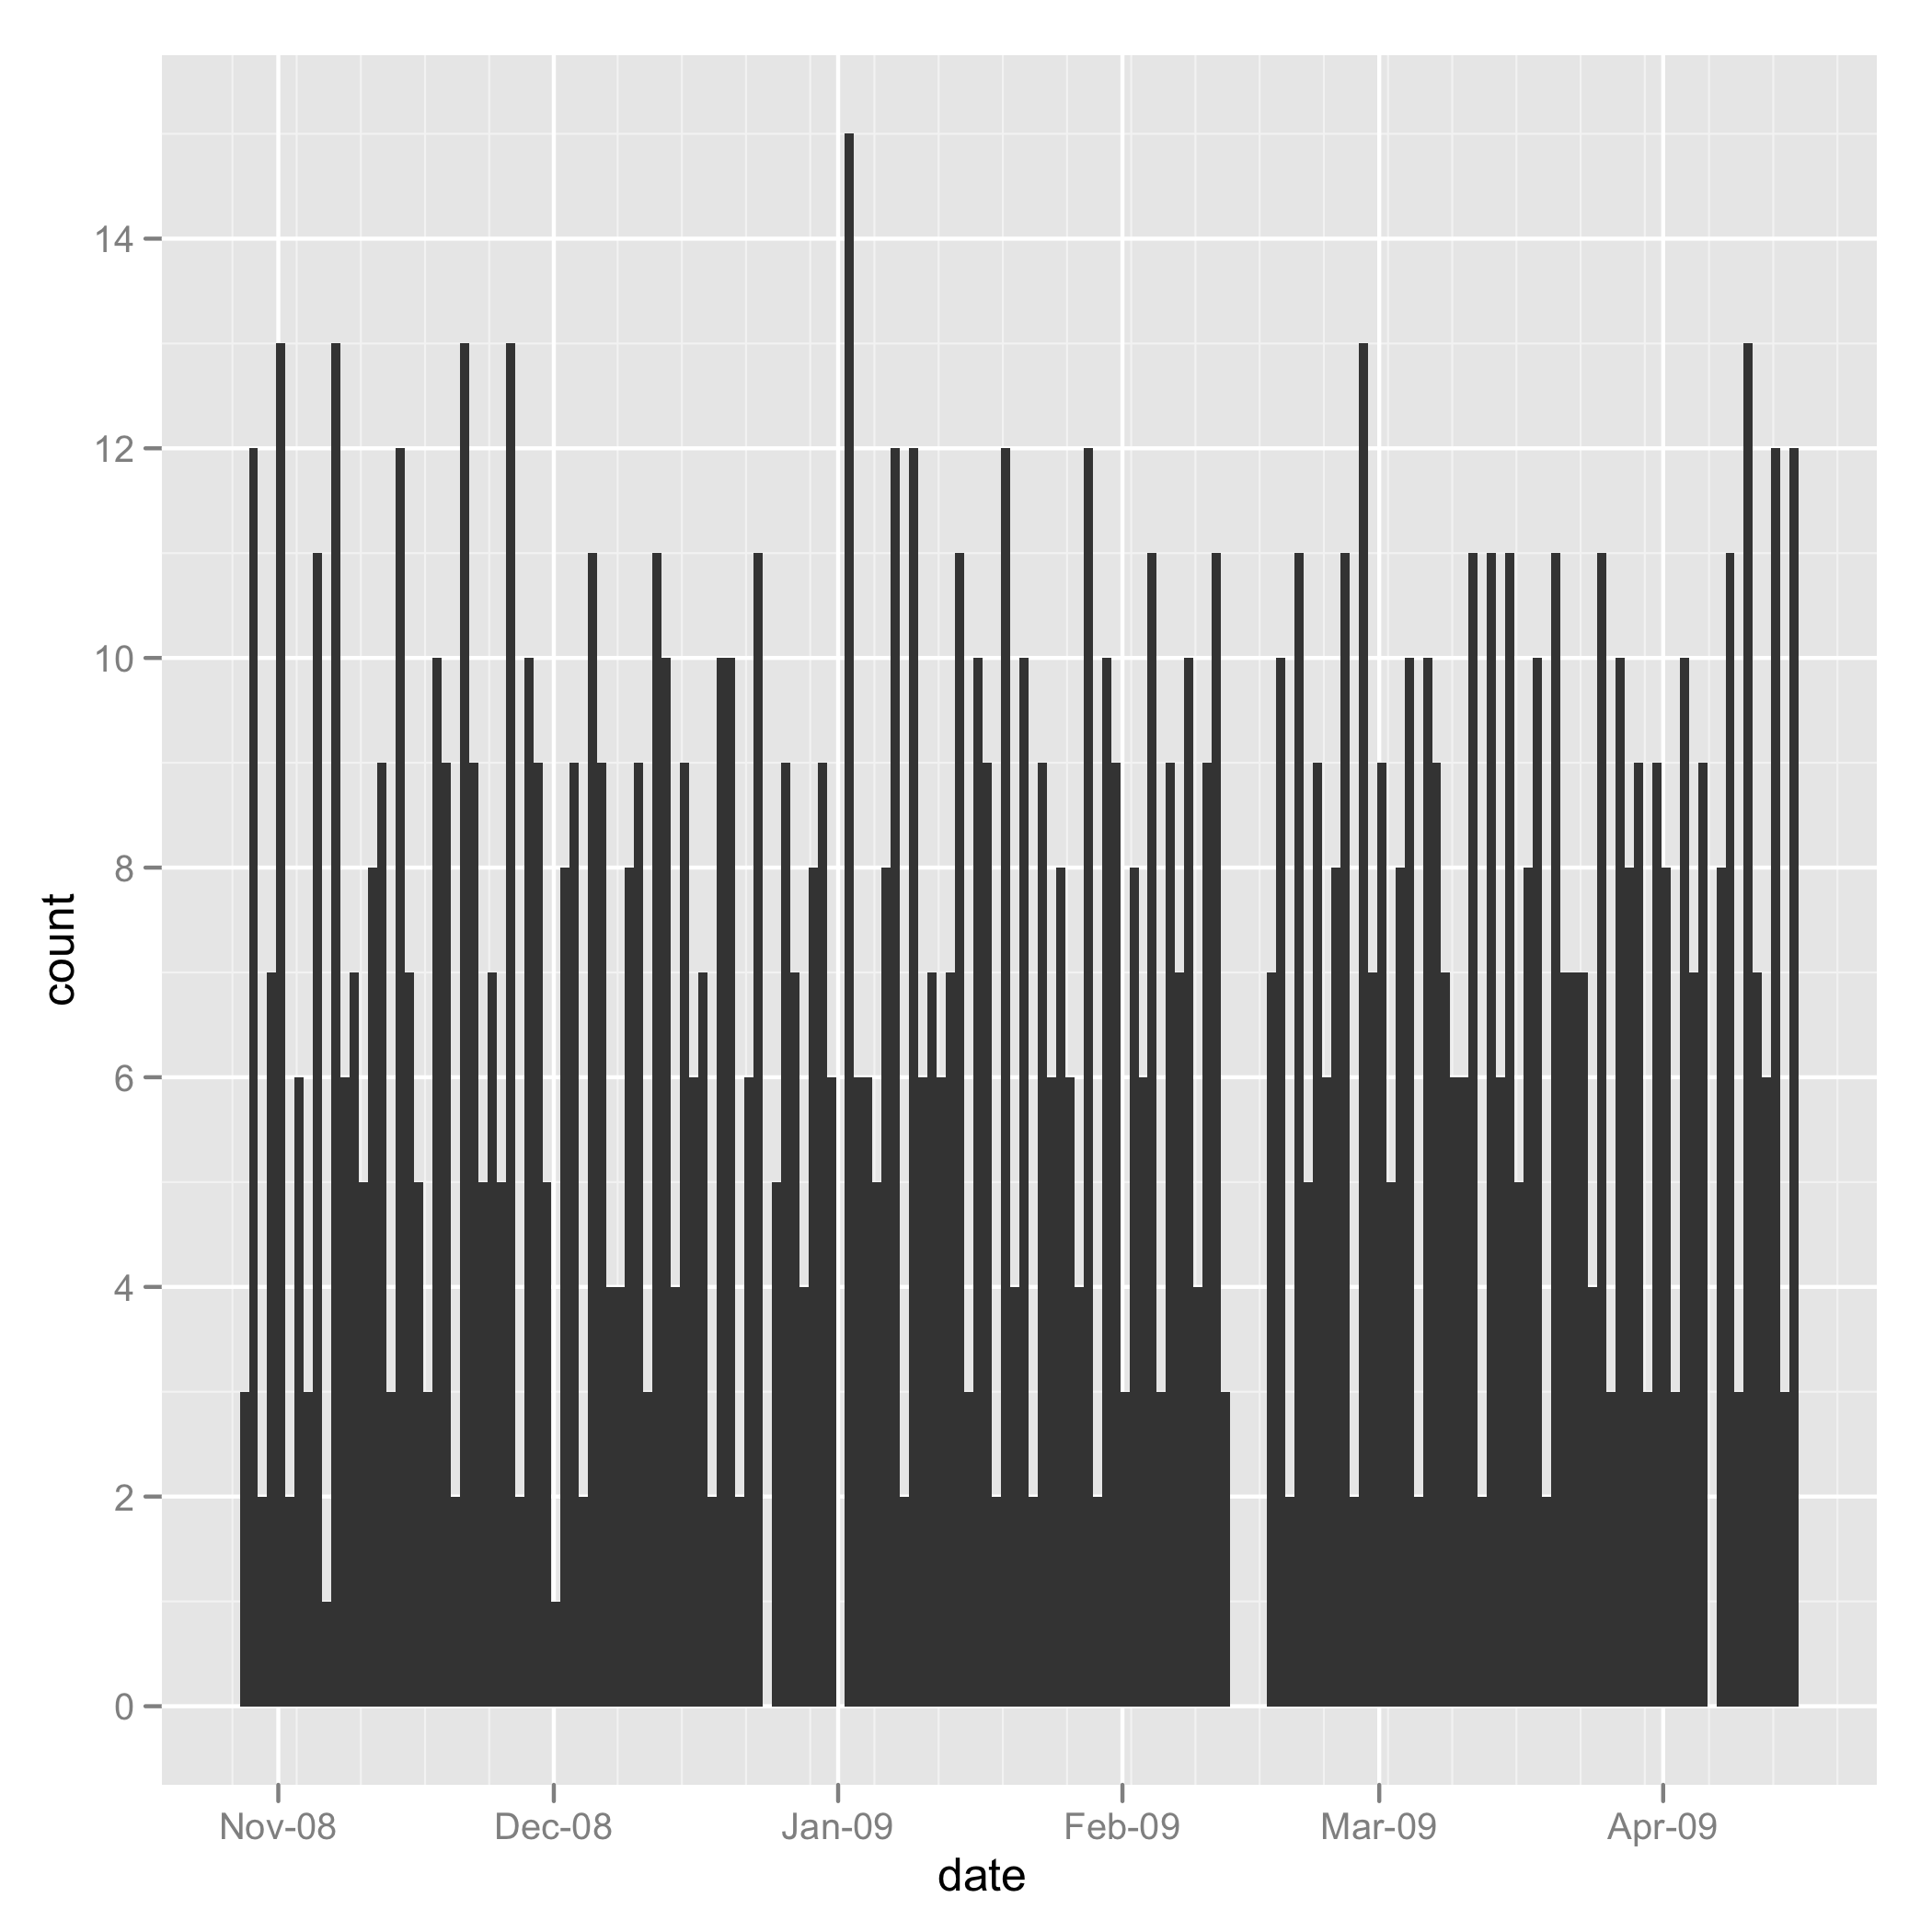
\includegraphics[width=.5\textwidth]{game-dates-histogram.png}        
  \caption{Number of games played per date}
  \label{fig:games-date}
\end{figure}

Figure~\ref{fig:games-date} shows that games are played continuously throughout the season with one short break and a few one day breaks, which may be holidays. The histogram also reveals a cyclic pattern to the data. We can investigate this pattern by looking at the weekdays on which each game is played. \\

\code{R> qplot(wday(date), data = basketball, geom = "histogram")}\\

\begin{figure}[htpb]
  \centering
  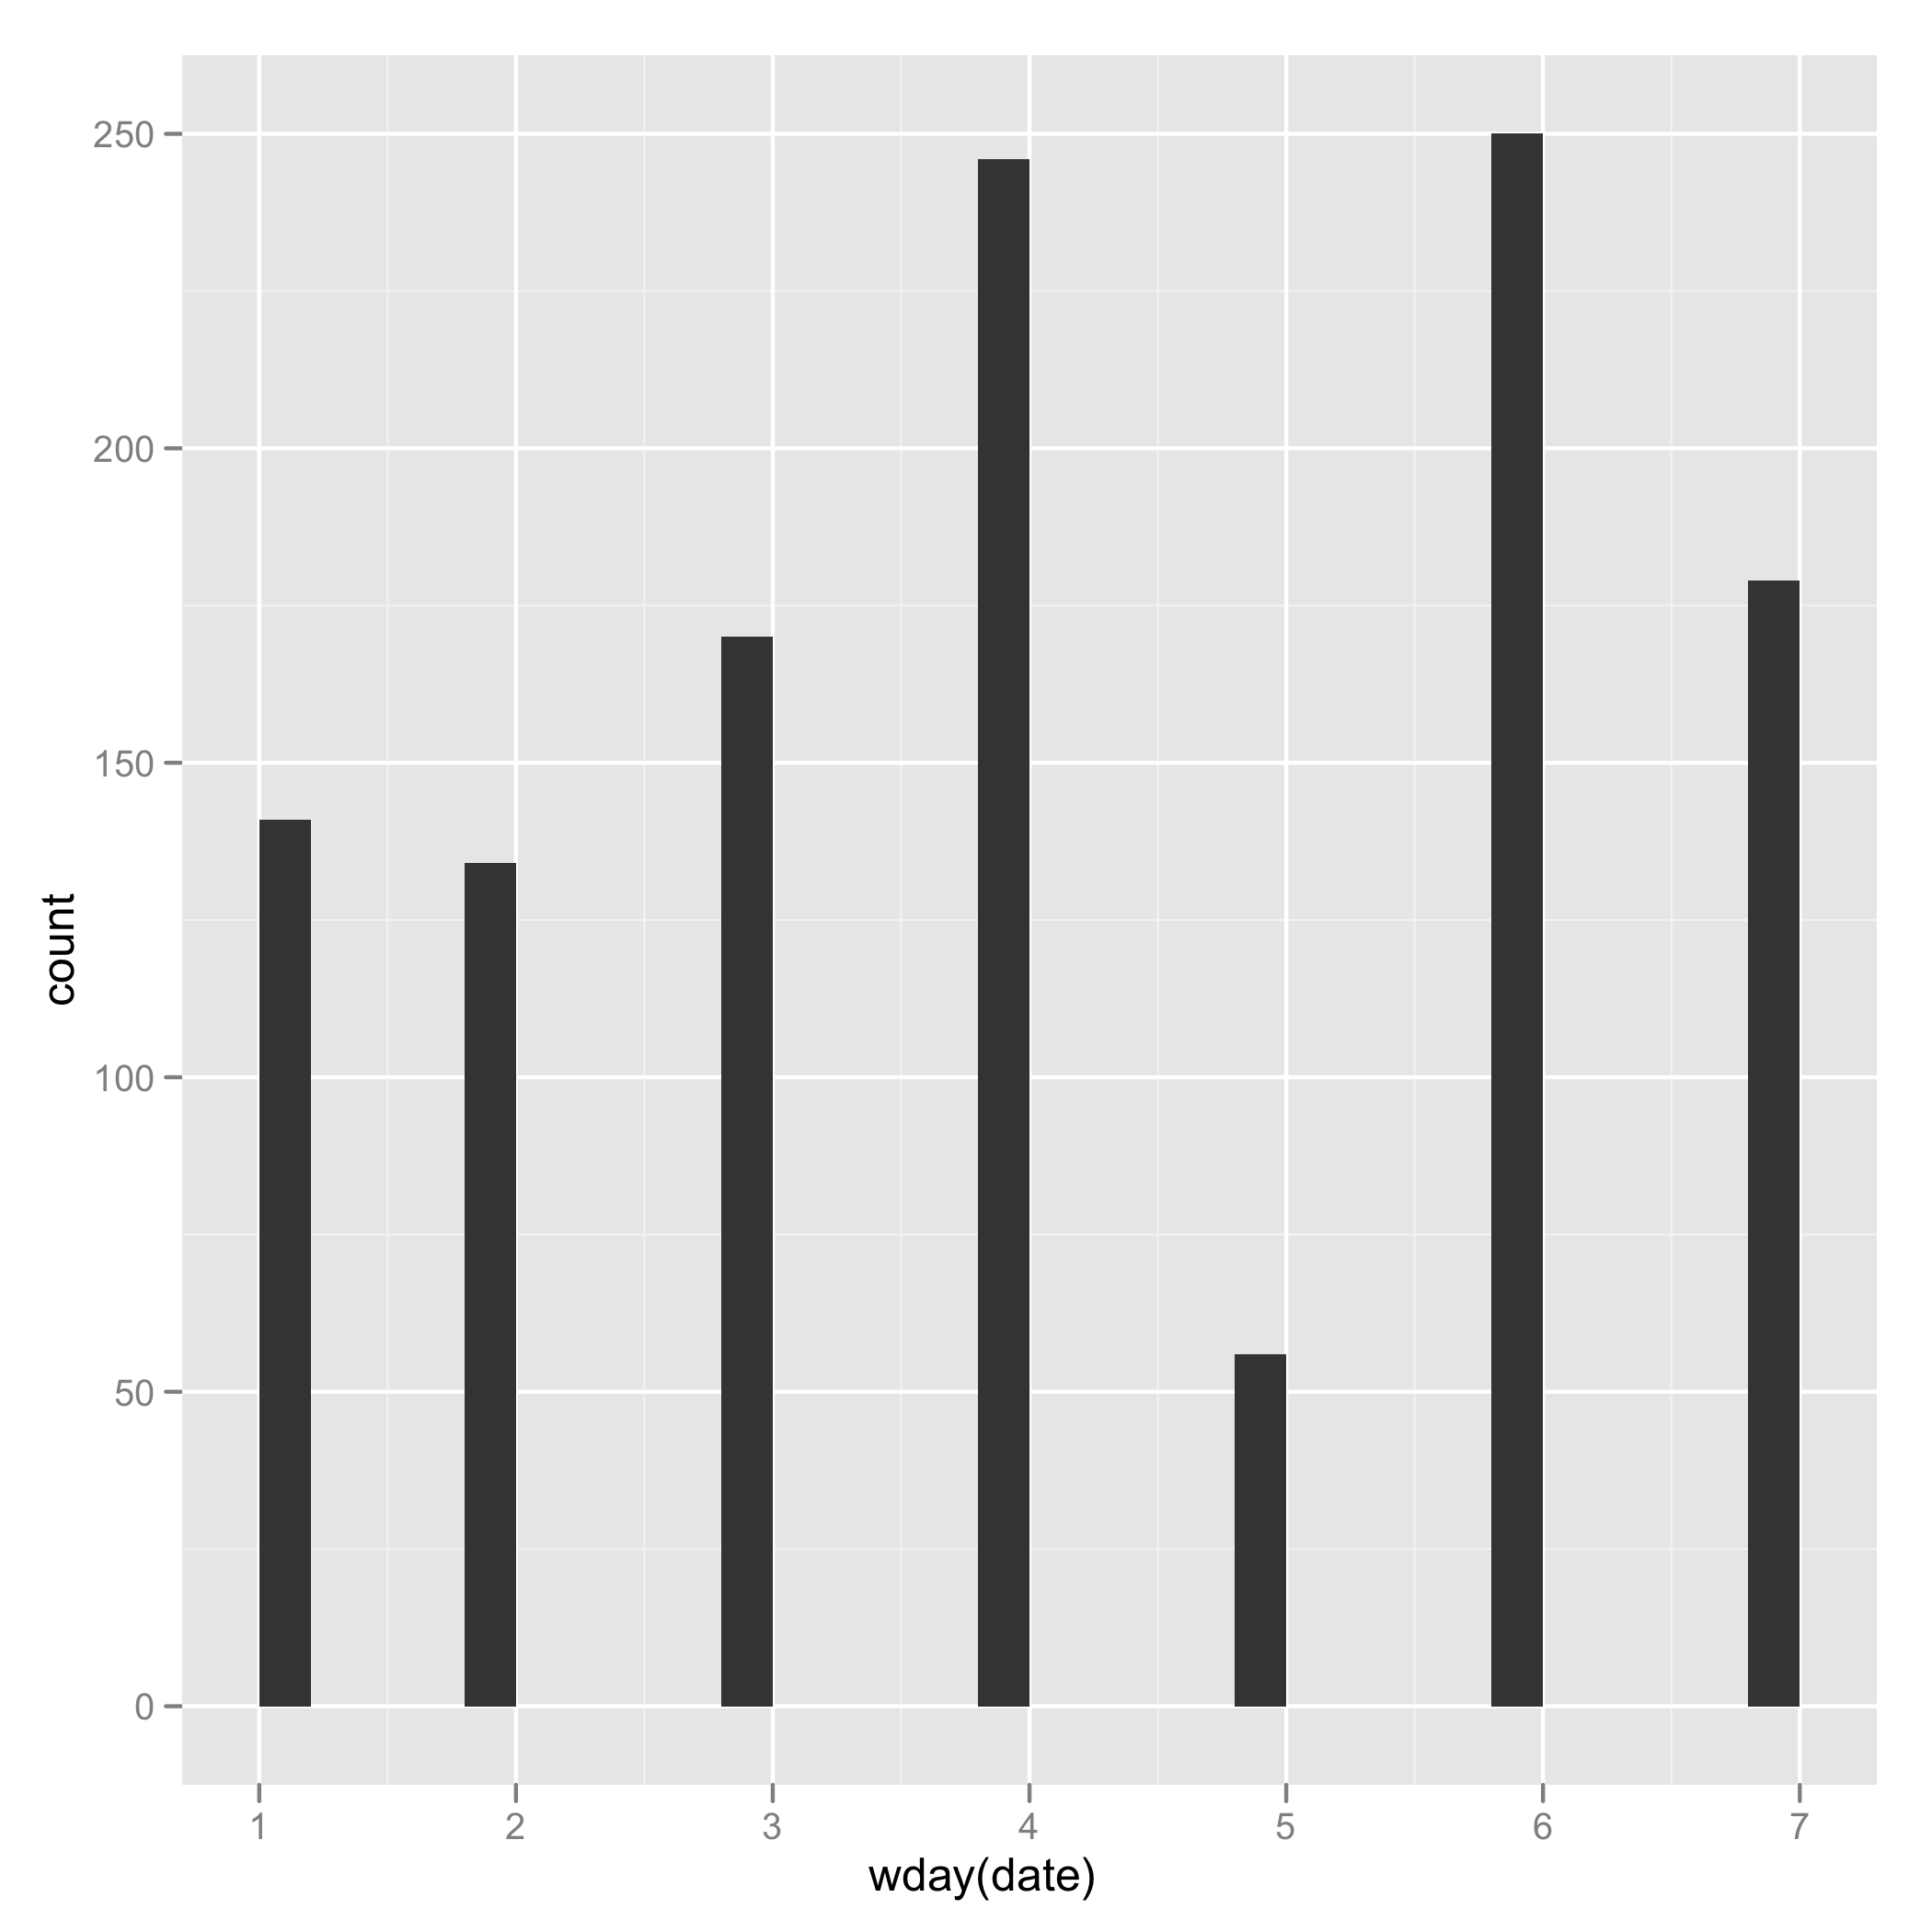
\includegraphics[width=.49\textwidth]{game-days-histogram.png}    
    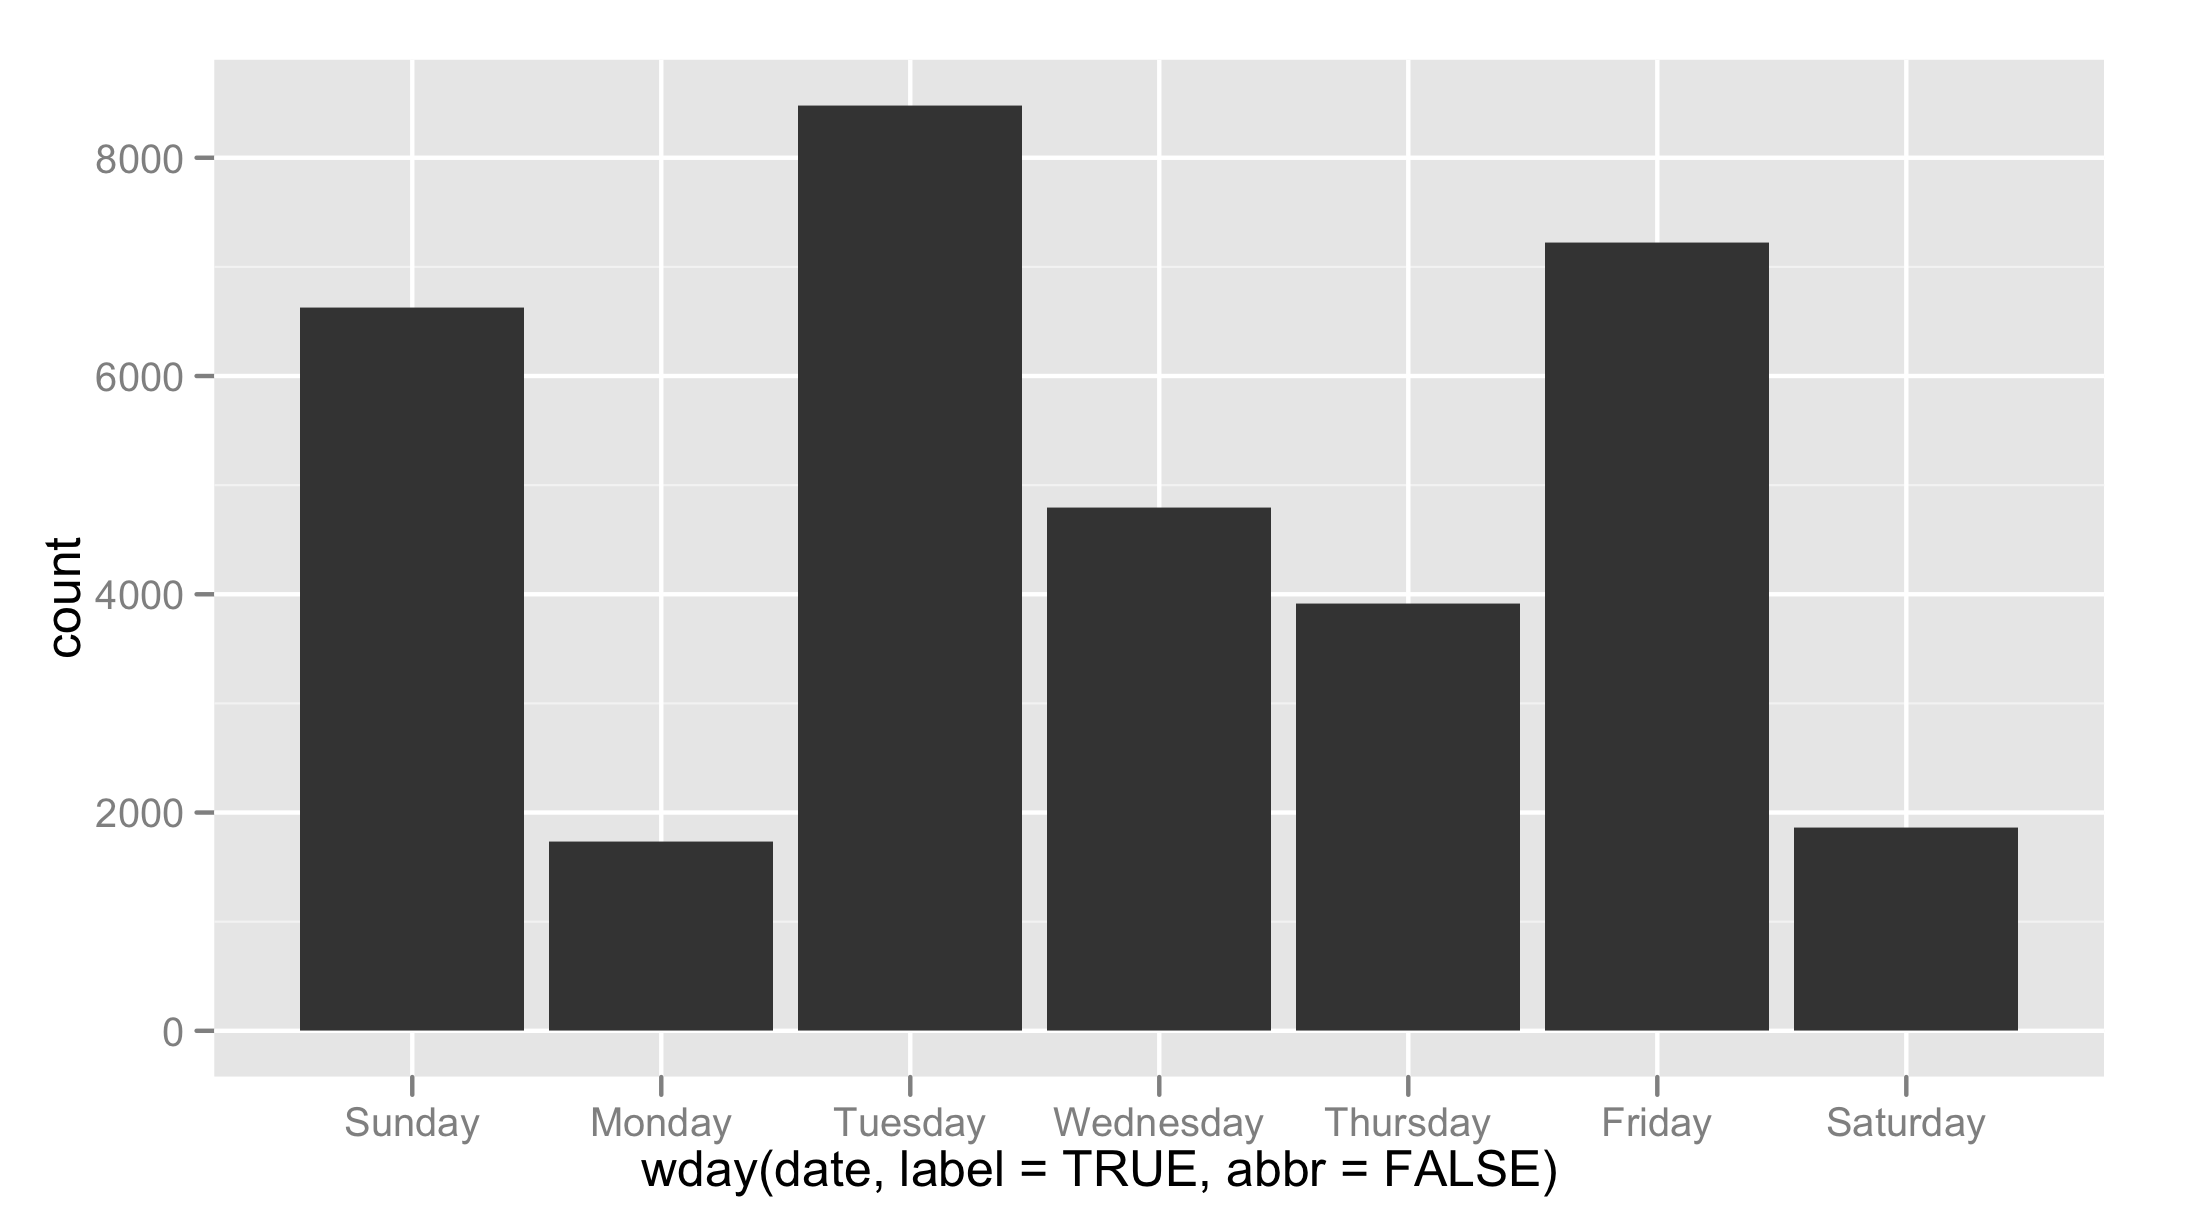
\includegraphics[width=.49\textwidth]{weekdays-histogram.png}     
  \caption{Number of games played per weekday}
  \label{fig:games-days}
\end{figure}


\emph{Note: this is better accomplished with the non-lubridate function qplot(weekdays(date), data = basketball, geom = ``histogram"), shown on right}\\

The frequency of basketball games appears to vary throughout the week, figure~\ref{fig:games-days}. Surprisingly, the most games are played on Fridays and on Wednesdays.\\

Now let's look at the games themselves. In particular, let's look at the time until the first score is made. 

\emph{Note this required manipulating the data set so much with plyr, that it would appear rather complicated if I listed all of the script here.}


\code{R> qplot(time, data = first_play, geom = "histogram", binwidth = 2)}\\

\begin{figure}[htpb]
  \centering
  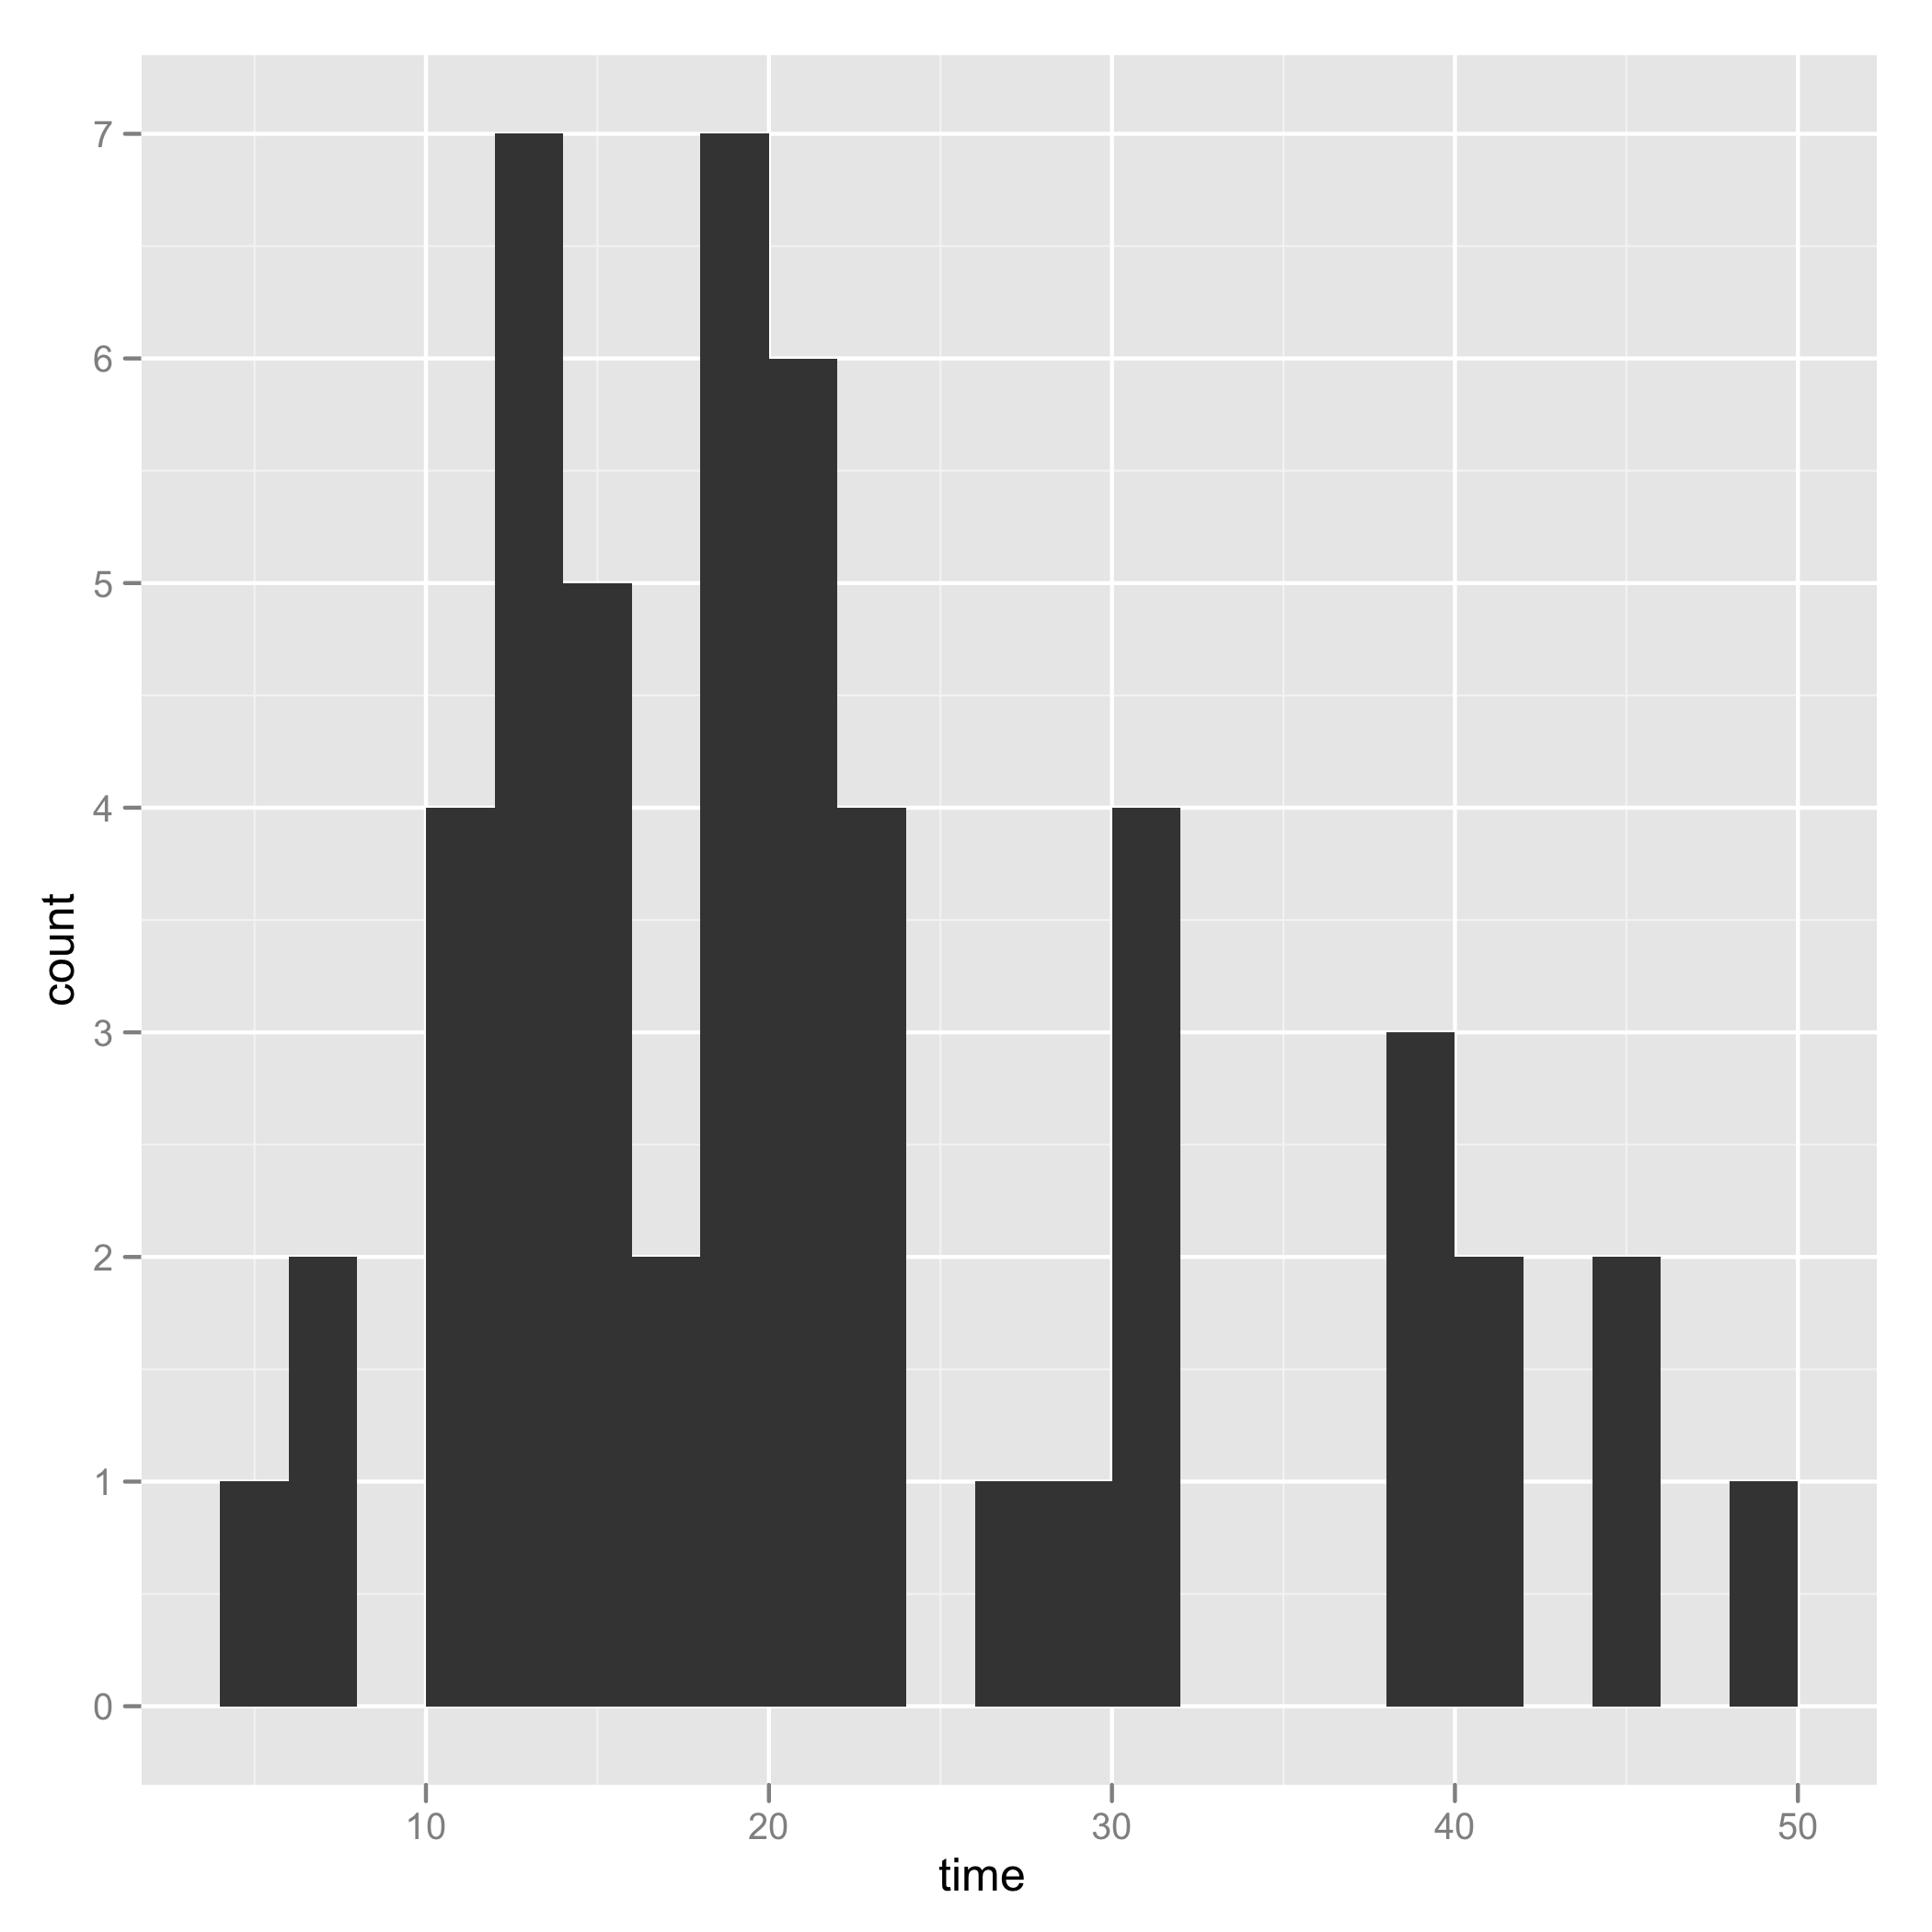
\includegraphics[width=.5\textwidth]{seconds-til-first-score.png}        
  \caption{Seconds until first score of game}
  \label{fig:first-score}
\end{figure}

We see that the first points of each game are usually made within the first 30 seconds, figure~\ref{fig:first-score}. The longest time until the first score was 50 seconds. Moreover, the distribution of time until the first score is bimodal. Perhaps the first mode shows games where the first team to control the ball scored and the second mode shows games where the first team to control the ball missed and the second team scored.



\section*{Acknowledgements}
I'd like to thank the National Science Foundation. This work was supported by the NSF under Grant WHAT GRANT NUMBER? 
% Acknowledge NSF grant here, since it paid for your summer.

\section*{References}

\end{document}
